\documentclass[14pt,a4paper]{article}

% =================== PACOTES ===================
\usepackage[utf8]{inputenc}
\usepackage[T1]{fontenc}
\usepackage[brazil]{babel}
\usepackage{graphicx}   % para inserir o logo
\usepackage{setspace}   % espaçamento
\usepackage{geometry}   % margens
\usepackage{tcolorbox}  % caixas de solução
\usepackage{fancyhdr}   % cabeçalho e rodapé
\usepackage{float}
\usepackage{caption}
\tcbuselibrary{theorems}
\usepackage{listings}   % Para exibir código fonte
\usepackage{xcolor}

\geometry{a4paper, top=3cm, bottom=2.5cm, left=3cm, right=2.5cm}

% =================== CABEÇALHO ===================
\pagestyle{fancy}
\fancyhf{}
\fancyhead[L]{Maykon Hopka -- 23203081}  
\fancyfoot[C]{\thepage}

% =================== AMBIENTE DE SOLUÇÃO ===================
\newtcbtheorem[number within=section]{solucao}{Solução}%
{colback=green!5,colframe=green!60!black,fonttitle=\bfseries}{sol}

% =================== CAPA ===================
\begin{document}
\begin{titlepage}
    \centering
    
    
\includegraphics[width=0.25\textwidth]{logo_ufsc.png}\par\vspace{1cm}
    
    {\Large\bfseries Universidade Federal de Santa Catarina \par}
    \vspace{0.5cm}
    {\large Centro de Engenharias da Mobilidade \par}
    {\large Curso de Engenharia Mecatrônica \par}
    \vfill
    
    {\Huge\bfseries Impasses \par}
    \vspace{0.5cm}
    {\Large Disciplina: Sistemas Operacionais\par}
    \vspace{0.3cm}
    {\large Aluno: Maykon Hopka \par}
    \vfill
    
    {\large Joinville – 2025}
\end{titlepage}

% =================== CONTEÚDO ===================
\section{Exercícios}

\subsection*{Exercício 1}
Analisar e apontar quais são as regiões críticas do código sujeitas a condição de corrida.

\begin{solucao}{Exercício 1}{}
A região crítica ocorre dentro da função \texttt{ThreadAdd}, especificamente nas instruções que leem, incrementam e escrevem o valor da variável global \texttt{count}:

\begin{itemize}
    \item \texttt{tmp = count;}
    \item \texttt{tmp = tmp + 1;}
    \item \texttt{count = tmp;}
\end{itemize}

\end{solucao}

\subsection*{Exercício 2}
Mostrar que o resultado da execução é sujeito a condição de corrida.

\begin{solucao}{Exercício 2}{}
Executando o programa original (sem uso de mutex), é possível observar que o valor final de \texttt{count} nem sempre atinge o esperado \texttt{2 * NITER}. Um exemplo de saída:

\begin{verbatim}
$ ./sem_mutex
BOOM! count is [1724351217], should be 2000000000
\end{verbatim}

Isso demonstra que houve **perda de incremento** devido à interferência entre as duas threads que acessam \texttt{count} simultaneamente.
\end{solucao}

\newpage

\subsection*{Exercício 3}
Implementar a técnica de sincronização apropriada para resolver a condição de corrida.

\begin{center}
        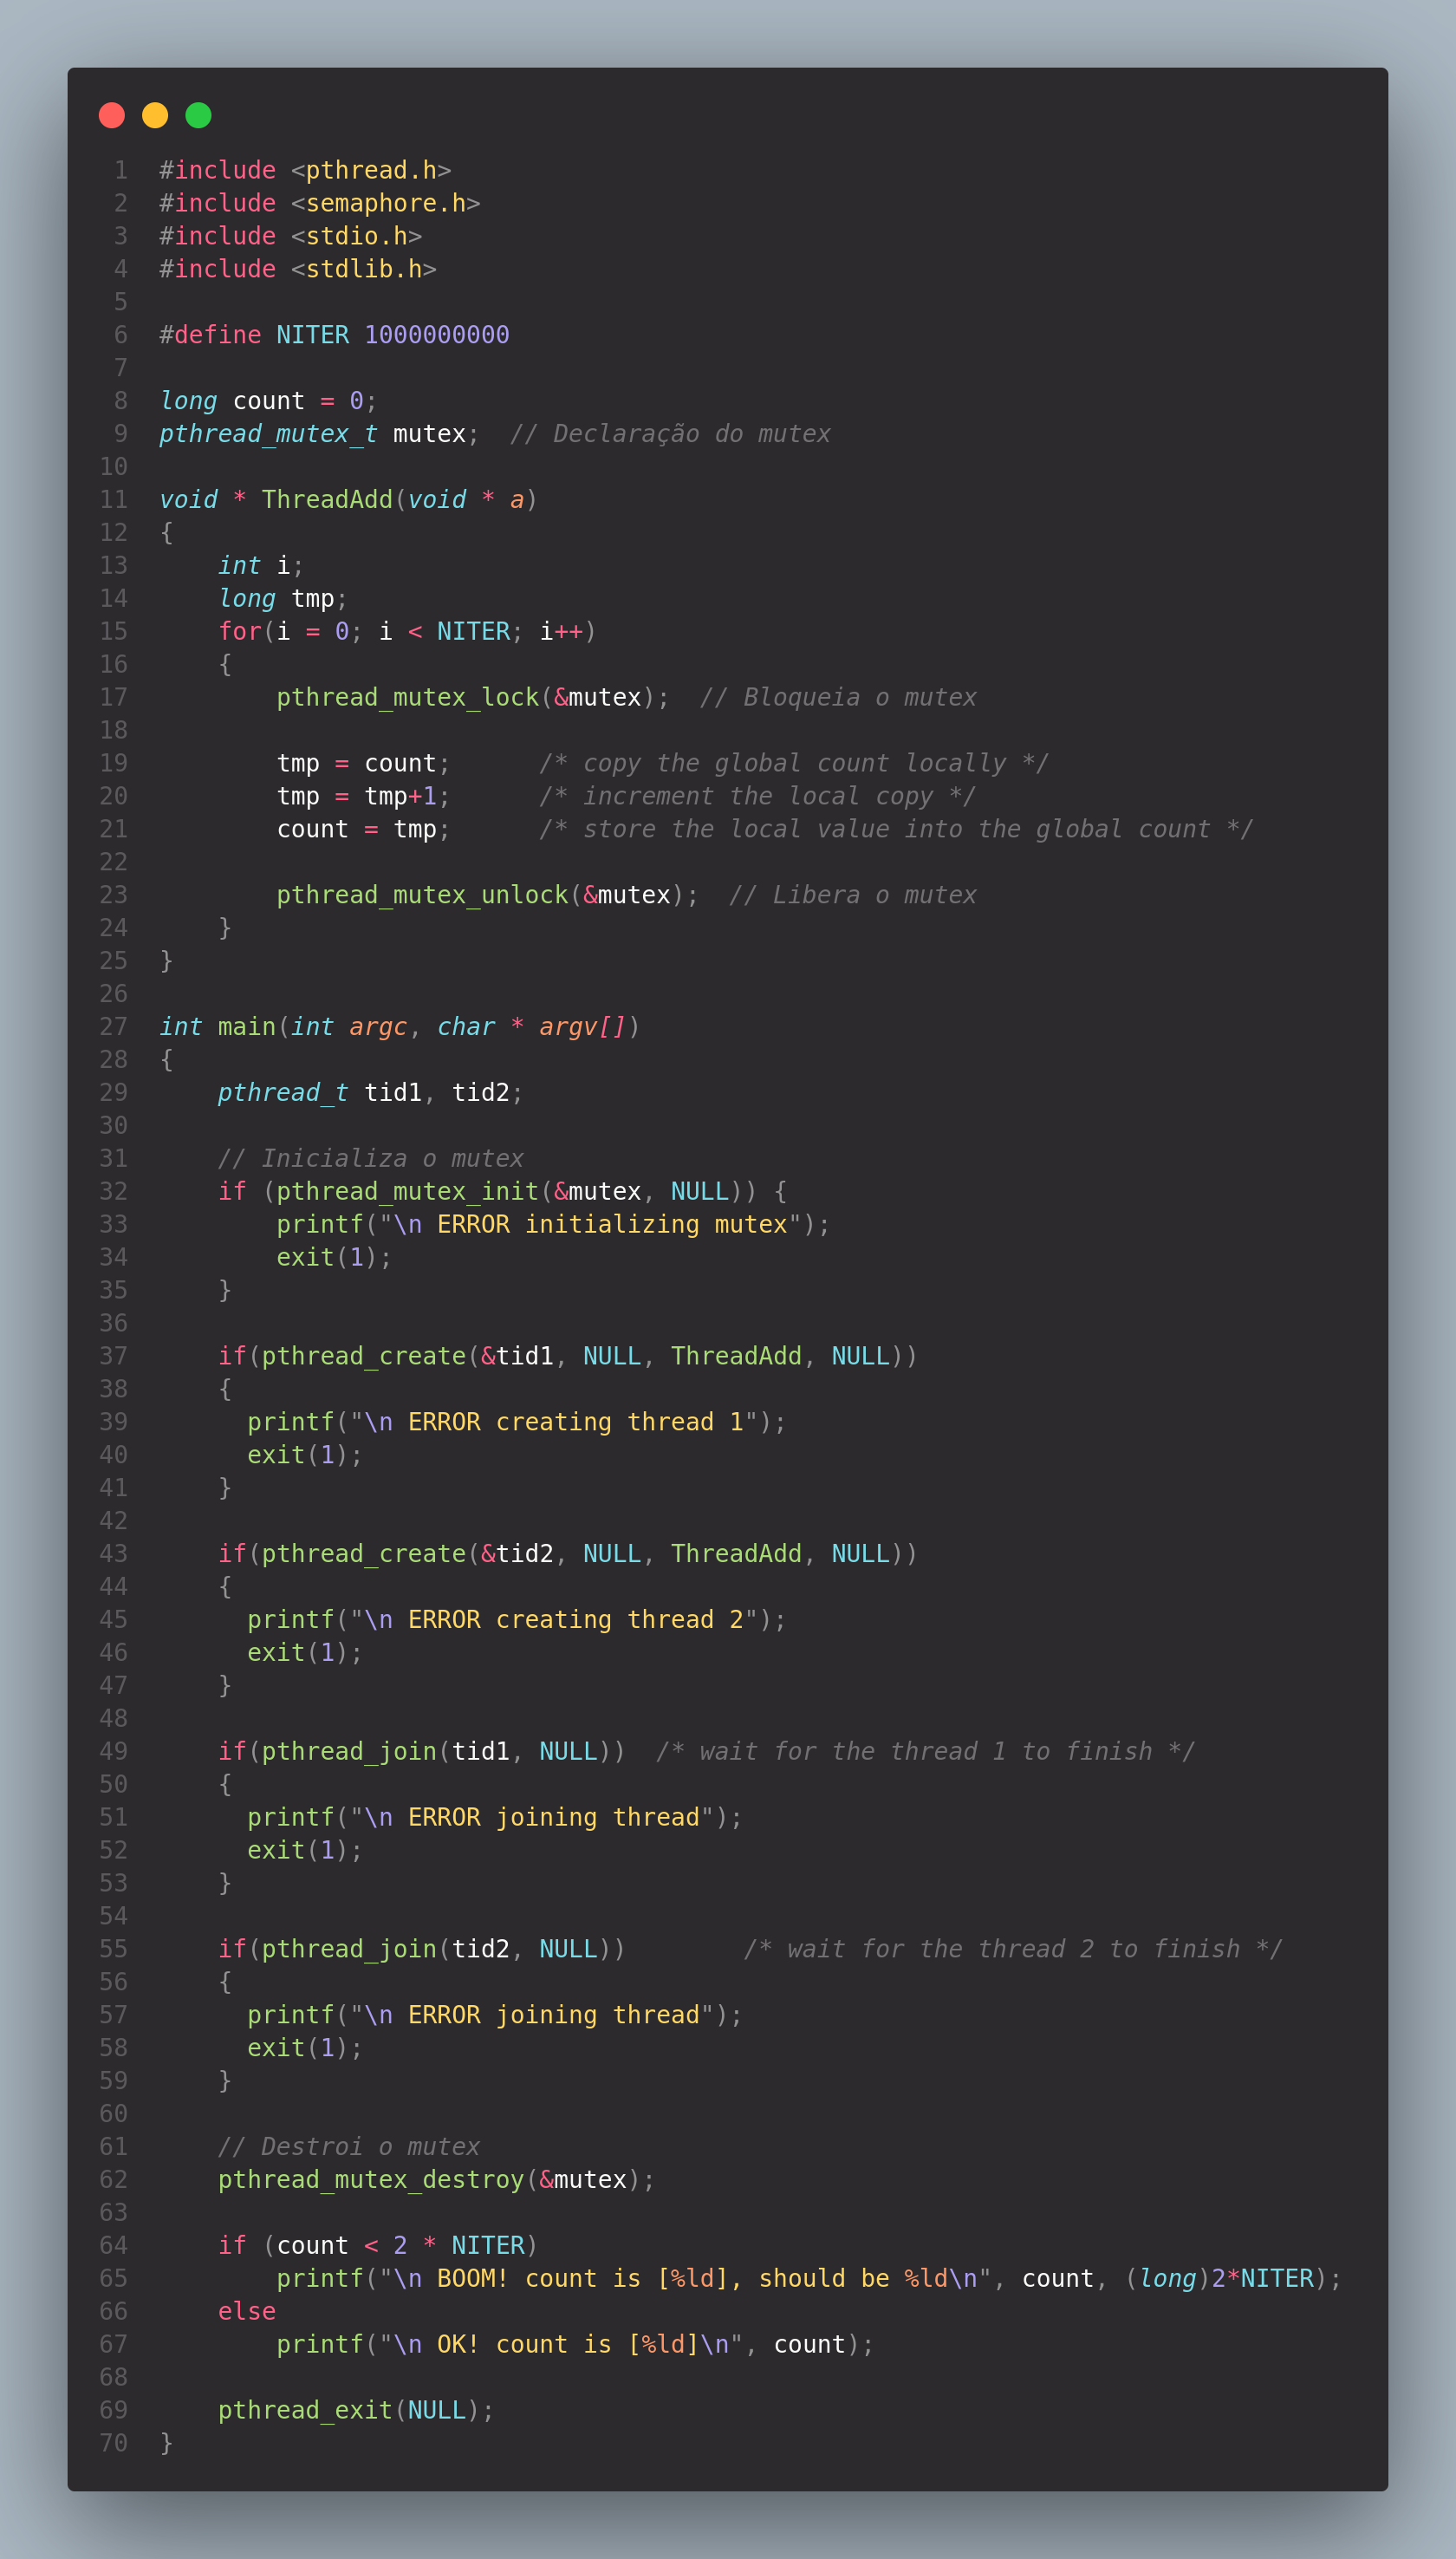
\includegraphics[width=0.8\textwidth]{code.png}
        \captionof{figure}{código com mutex para evitar condição de corrida}
    \end{center}
% =================== FIM ===================

\end{document}
